\section{Phương pháp giải quyết}

Chương này trình bày chi tiết phương pháp luận và các bước thực hiện để giải quyết bài toán phân tích mối liên hệ giao thông giữa các nút quan trọng tại TP.HCM. Phương pháp được thiết kế dựa trên nền tảng lý thuyết đã trình bày ở Chương 2 và các khoảng trống nghiên cứu được xác định ở Chương 3, đồng thời tận dụng dữ liệu lịch sử từ TomTom Historical Traffic Stats API.

\subsection{Tổng quan phương pháp tiếp cận}

\subsubsection{Định hướng giải pháp}

Để giải quyết bài toán phân tích mối liên hệ và lan truyền tắc nghẽn giữa các nút giao thông, đề tài đề xuất một pipeline xử lý toàn diện kết hợp nhiều kỹ thuật từ Big Data, Deep Learning, và phân tích thống kê. Giải pháp tập trung vào ba mục tiêu chính:

\begin{enumerate}
    \item \textbf{Phát hiện tương quan không gian-thời gian}: Xác định các cặp nút giao thông có mức độ ảnh hưởng lẫn nhau cao, định lượng độ mạnh của mối tương quan và xác định độ trễ lan truyền.
    
    \item \textbf{Xác định quan hệ nhân quả}: Phân biệt mối tương quan đơn thuần và quan hệ nhân-quả thực sự, xác định nút nào là nguyên nhân gây ra tắc nghẽn lan truyền.
    
    \item \textbf{Dự báo lan truyền tắc nghẽn}: Xây dựng mô hình có khả năng dự báo khi một nút giao thông bị tắc nghẽn sẽ lan truyền đến các nút nào và trong bao lâu.
\end{enumerate}

\subsubsection{Kiến trúc tổng thể}

Hệ thống được thiết kế theo kiến trúc phân tầng, mỗi tầng đảm nhiệm một nhóm chức năng cụ thể:

\begin{figure}[h]
\centering
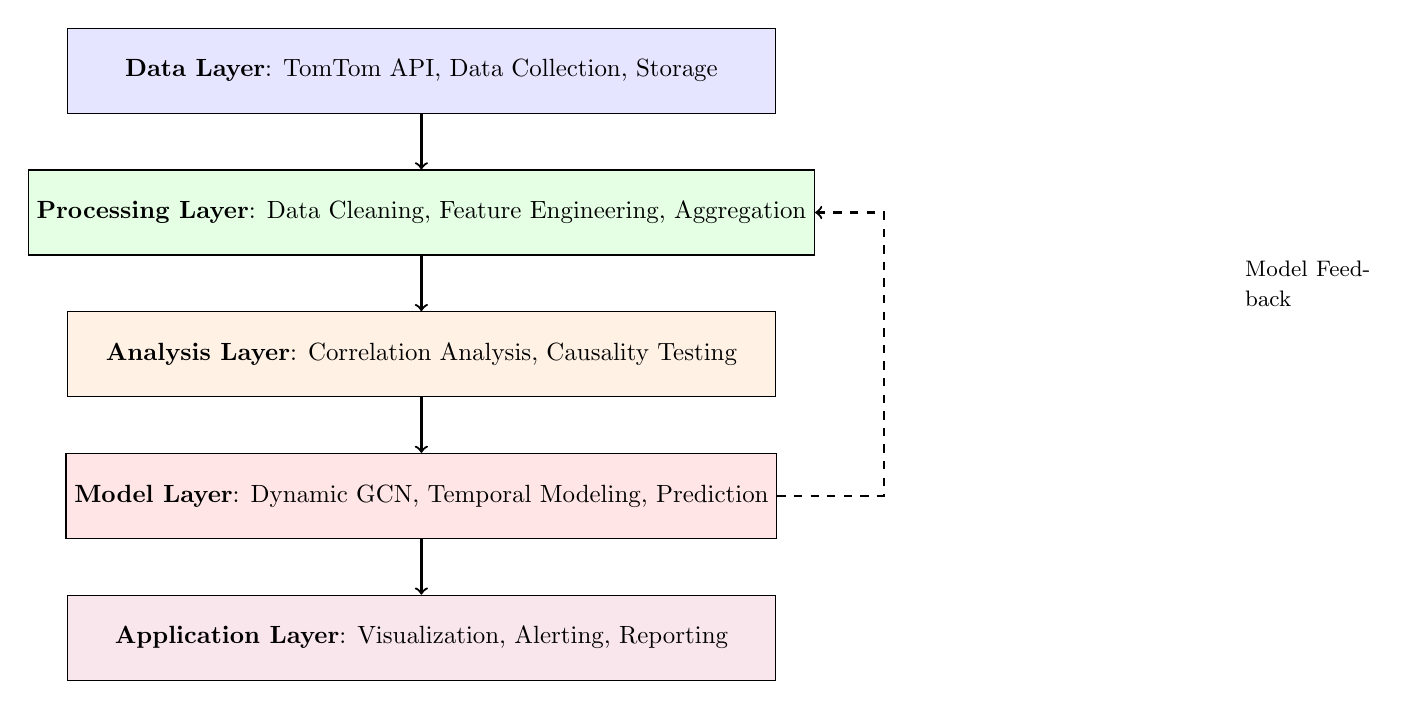
\begin{tikzpicture}[node distance=1.5cm, scale=0.9, transform shape]
% Data Layer
\node[draw, rectangle, minimum width=10cm, minimum height=1.2cm, fill=blue!10] (data) {
    \textbf{Data Layer}: TomTom API, Data Collection, Storage
};

% Processing Layer
\node[draw, rectangle, minimum width=10cm, minimum height=1.2cm, fill=green!10, below of=data, yshift=-0.5cm] (processing) {
    \textbf{Processing Layer}: Data Cleaning, Feature Engineering, Aggregation
};

% Analysis Layer
\node[draw, rectangle, minimum width=10cm, minimum height=1.2cm, fill=orange!10, below of=processing, yshift=-0.5cm] (analysis) {
    \textbf{Analysis Layer}: Correlation Analysis, Causality Testing
};

% Model Layer
\node[draw, rectangle, minimum width=10cm, minimum height=1.2cm, fill=red!10, below of=analysis, yshift=-0.5cm] (model) {
    \textbf{Model Layer}: Dynamic GCN, Temporal Modeling, Prediction
};

% Application Layer
\node[draw, rectangle, minimum width=10cm, minimum height=1.2cm, fill=purple!10, below of=model, yshift=-0.5cm] (app) {
    \textbf{Application Layer}: Visualization, Alerting, Reporting
};

% Arrows
\draw[->, thick] (data) -- (processing);
\draw[->, thick] (processing) -- (analysis);
\draw[->, thick] (analysis) -- (model);
\draw[->, thick] (model) -- (app);

% Feedback loop
\draw[->, thick, dashed] (model.east) -- ++(1.5,0) |- (processing.east);
\node[right, text width=2cm] at (11.5, -3) {\small Model Feedback};

\end{tikzpicture}
\caption{Kiến trúc tổng thể hệ thống}
\label{fig:overall_architecture}
\end{figure}

\subsubsection{Quy trình xử lý chính}

Pipeline xử lý dữ liệu và phân tích được thực hiện theo trình tự sau:

\begin{enumerate}
    \item \textbf{Thu thập dữ liệu}: Lấy dữ liệu lịch sử từ TomTom API cho các nút giao thông được chọn
    \item \textbf{Tiền xử lý}: Làm sạch, chuẩn hóa, và xử lý missing values
    \item \textbf{Trích xuất đặc trưng}: Tính toán các đặc trưng giao thông và thời gian
    \item \textbf{Phân tích tương quan}: Xác định mối tương quan không gian-thời gian
    \item \textbf{Kiểm định nhân quả}: Áp dụng Granger Causality Test
    \item \textbf{Xây dựng đồ thị động}: Tạo ma trận kề thay đổi theo thời gian
    \item \textbf{Huấn luyện mô hình}: Phát triển mô hình dự báo dựa trên GNN
    \item \textbf{Đánh giá và triển khai}: Kiểm thử và tích hợp vào hệ thống
\end{enumerate}

\newpage
\subsection{Thu thập và chuẩn bị dữ liệu}

\subsubsection{Nguồn dữ liệu: TomTom Historical Traffic Stats}

\subsubsubsection{Lý do lựa chọn TomTom API}

Dữ liệu giao thông lịch sử từ TomTom được lựa chọn làm nguồn dữ liệu chính cho đề tài vì các lý do sau:

\begin{itemize}
    \item \textbf{Độ phủ toàn diện}: TomTom cung cấp dữ liệu cho hầu hết các tuyến đường chính tại TP.HCM, bao gồm cả các khu vực trung tâm và vùng ven.
    
    \item \textbf{Chất lượng dữ liệu}: Dữ liệu được tổng hợp từ nhiều nguồn (GPS probe data, cảm biến, crowdsourcing) và đã qua xử lý, lọc nhiễu bởi TomTom.
    
    \item \textbf{Dữ liệu lịch sử dài hạn}: API cung cấp dữ liệu lịch sử từ nhiều tháng đến nhiều năm, đủ để huấn luyện mô hình học sâu.
    
    \item \textbf{Độ phân giải thời gian phù hợp}: Dữ liệu có độ phân giải 5 phút, cân bằng giữa chi tiết và khả năng xử lý.
    
    \item \textbf{Các chỉ số phong phú}: Bao gồm tốc độ thực tế, tốc độ tự do, thời gian di chuyển, độ tin cậy, giúp phân tích đa chiều.
\end{itemize}

\subsubsubsection{Cấu trúc dữ liệu TomTom}

TomTom Historical Traffic Stats API cung cấp dữ liệu theo cấu trúc sau:

\begin{itemize}
    \item \textbf{Road Segments}: Mỗi đoạn đường được định danh bởi segment ID duy nhất
    \item \textbf{Temporal Resolution}: Dữ liệu theo khung thời gian 5 phút
    \item \textbf{Speed Metrics}:
    \begin{itemize}
        \item \texttt{currentSpeed}: Tốc độ trung bình thực tế (km/h)
        \item \texttt{freeFlowSpeed}: Tốc độ tự do khi không có tắc nghẽn (km/h)
        \item \texttt{confidence}: Độ tin cậy của số liệu (0-1)
    \end{itemize}
    \item \textbf{Congestion Indicators}:
    \begin{itemize}
        \item \texttt{travelTime}: Thời gian di chuyển thực tế (giây)
        \item \texttt{freeFlowTravelTime}: Thời gian di chuyển lý tưởng (giây)
    \end{itemize}
    \item \textbf{Metadata}: Thông tin đoạn đường (tên đường, tọa độ, chiều dài)
\end{itemize}

\subsubsection{Lựa chọn nút giao thông nghiên cứu}

\subsubsubsection{Tiêu chí lựa chọn}

Việc lựa chọn các nút giao thông để nghiên cứu dựa trên các tiêu chí sau:

\begin{enumerate}
    \item \textbf{Tầm quan trọng chiến lược}:
    \begin{itemize}
        \item Nút nằm trên các tuyến huyết mạch nối các quận trung tâm
        \item Cổng vào/ra khu vực trung tâm TP.HCM
        \item Giao lộ có lưu lượng cao và thường xuyên ùn tắc
    \end{itemize}
    
    \item \textbf{Độ phủ dữ liệu}:
    \begin{itemize}
        \item Đảm bảo có dữ liệu TomTom liên tục cho đoạn đường
        \item Tỷ lệ missing data dưới 10\%
        \item Độ tin cậy trung bình (confidence) trên 0.7
    \end{itemize}
    
    \item \textbf{Tính đại diện}:
    \begin{itemize}
        \item Phân bố đều trong khu vực nghiên cứu
        \item Bao gồm nhiều loại đường: đại lộ, đường chính, đường nhánh
        \item Đa dạng về mật độ giao thông và đặc điểm vận hành
    \end{itemize}
    
    \item \textbf{Khả năng kết nối}:
    \begin{itemize}
        \item Có mối liên hệ trực tiếp hoặc gián tiếp với các nút khác
        \item Nằm trong cùng một mạng lưới liên thông
    \end{itemize}
\end{enumerate}

\subsubsubsection{Danh sách nút giao thông được chọn}

Dựa trên các tiêu chí trên, đề tài lựa chọn 20 nút giao thông trọng điểm tại TP.HCM, bao gồm:

\begin{table}[h]
\centering
\caption{Các nút giao thông được lựa chọn}
\begin{tabular}{|l|l|l|}
\hline
\textbf{STT} & \textbf{Tên nút/đường} & \textbf{Khu vực} \\ \hline
1 & Ngã ba Cách Mạng Tháng 8 - Điện Biên Phủ & Quận 3 \\ \hline
2 & Ngã tư Hàng Xanh & Quận Bình Thạnh \\ \hline
3 & Cầu Sài Gòn & Quận 1 - Quận 4 \\ \hline
4 & Đường Võ Văn Kiệt (đoạn Q1) & Quận 1 \\ \hline
5 & Ngã tư Bảy Hiền & Quận Tân Bình \\ \hline
6 & Xa lộ Hà Nội (đoạn Q9) & Quận 9 \\ \hline
7 & Đại lộ Võ Văn Kiệt (đoạn Q5) & Quận 5 \\ \hline
8 & Nguyễn Thị Minh Khai & Quận 1, Quận 3 \\ \hline
9 & Cầu Kênh Tẻ & Quận 1 - Quận 7 \\ \hline
10 & Đường 3 Tháng 2 & Quận 10, Quận 11 \\ \hline
... & ... & ... \\ \hline
\end{tabular}
\label{tab:selected_nodes}
\end{table}

\subsubsection{Quy trình thu thập dữ liệu}

\subsubsubsection{Thiết kế data pipeline}

Pipeline thu thập dữ liệu được thiết kế để đảm bảo tính ổn định, hiệu quả và khả năng mở rộng:

\begin{figure}[h]
\centering
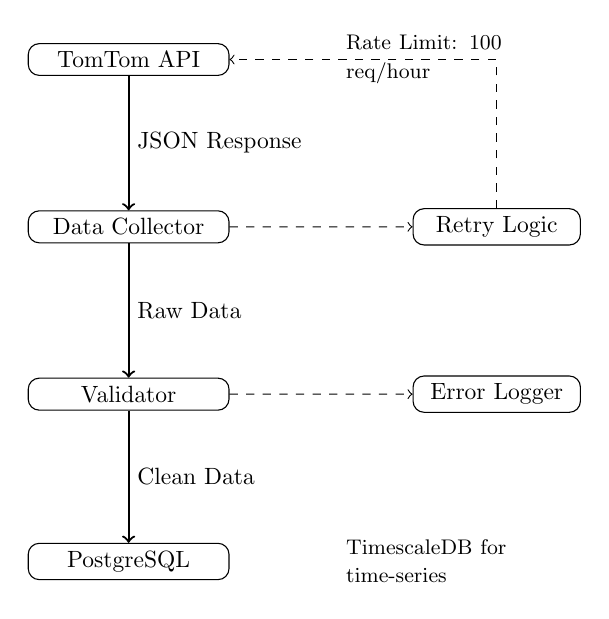
\begin{tikzpicture}[node distance=2.5cm, scale=0.85, transform shape]

% Nodes
\node[draw, rectangle, rounded corners, minimum width=3cm] (api) {TomTom API};
\node[draw, rectangle, rounded corners, minimum width=3cm, below of=api] (collector) {Data Collector};
\node[draw, rectangle, rounded corners, minimum width=3cm, below of=collector] (validator) {Validator};
\node[draw, rectangle, rounded corners, minimum width=3cm, below of=validator] (storage) {PostgreSQL};

% Parallel processes
\node[draw, rectangle, rounded corners, minimum width=2.5cm, right of=collector, xshift=3cm] (retry) {Retry Logic};
\node[draw, rectangle, rounded corners, minimum width=2.5cm, right of=validator, xshift=3cm] (logger) {Error Logger};

% Arrows
\draw[->, thick] (api) -- (collector) node[midway, right] {JSON Response};
\draw[->, thick] (collector) -- (validator) node[midway, right] {Raw Data};
\draw[->, thick] (validator) -- (storage) node[midway, right] {Clean Data};

\draw[->, dashed] (collector) -- (retry);
\draw[->, dashed] (retry) |- (api);
\draw[->, dashed] (validator) -- (logger);

% Labels
\node[right of=api, xshift=2cm, text width=2.5cm, align=left] {\small Rate Limit: 100 req/hour};
\node[right of=storage, xshift=2cm, text width=2.5cm, align=left] {\small TimescaleDB for time-series};

\end{tikzpicture}
\caption{Pipeline thu thập dữ liệu từ TomTom API}
\label{fig:data_collection_pipeline}
\end{figure}

\subsubsubsection{Các bước thu thập}

\begin{enumerate}
    \item \textbf{Xác định time range}:
    \begin{itemize}
        \item Thu thập dữ liệu từ 01-8-2024 đến 31-8-2024
        \item Độ phân giải: 5 phút/lần đo
        \item Tập trung vào giờ cao điểm: 6h-9h, 17h-20h
    \end{itemize}
    
    \item \textbf{API Request Strategy}:
    \begin{itemize}
        \item Batch requests để tối ưu số lần gọi API
        \item Implement exponential backoff khi gặp rate limit
        \item Cache responses để tránh duplicate requests
    \end{itemize}
    
    \item \textbf{Data Validation}:
    \begin{itemize}
        \item Kiểm tra completeness: đảm bảo đủ các trường bắt buộc
        \item Kiểm tra consistency: tốc độ không âm, trong giới hạn hợp lý
        \item Kiểm tra temporal continuity: không có gaps lớn giữa các measurements
    \end{itemize}
    
    \item \textbf{Error Handling}:
    \begin{itemize}
        \item Log tất cả errors để phân tích sau
        \item Retry failed requests với backoff strategy
        \item Alert khi error rate vượt threshold
    \end{itemize}
\end{enumerate}

\subsubsection{Tiền xử lý dữ liệu}

\subsubsubsection{Xử lý missing values}

Dữ liệu giao thông thực tế thường có missing values do nhiều nguyên nhân: lỗi cảm biến, mất kết nối, hoặc không đủ probe data. Chiến lược xử lý:

\begin{enumerate}
    \item \textbf{Phân loại missing patterns}:
    \begin{itemize}
        \item \textit{MCAR (Missing Completely At Random)}: Xảy ra ngẫu nhiên
        \item \textit{MAR (Missing At Random)}: Phụ thuộc vào biến quan sát được
        \item \textit{MNAR (Missing Not At Random)}: Phụ thuộc vào giá trị bị missing
    \end{itemize}
    
    \item \textbf{Phương pháp imputation}:
    \begin{itemize}
        \item \textbf{Linear Interpolation}: Cho gaps nhỏ (< 3 time steps)
        \[
        v_t = v_{t-1} + \frac{v_{t+k} - v_{t-1}}{k+1}
        \]
        
        \item \textbf{Seasonal Decomposition}: Cho gaps trung bình
        \[
        v_t = \text{trend}_t + \text{seasonal}_t + \text{residual}_t
        \]
        
        \item \textbf{KNN Imputation}: Dựa vào các nút láng giềng tương tự
        \[
        v_t^i = \frac{1}{k}\sum_{j \in \text{KNN}(i)} v_t^j \cdot w_{ij}
        \]
        
        \item \textbf{Deep Learning Imputation}: Sử dụng LSTM autoencoder cho gaps lớn
    \end{itemize}
    
    \item \textbf{Quality threshold}:
    \begin{itemize}
        \item Loại bỏ nút có > 20\% missing data
        \item Đánh dấu imputed values để đánh giá độ tin cậy
    \end{itemize}
\end{enumerate}

\subsubsubsection{Outlier detection và xử lý}

Outliers trong dữ liệu giao thông có thể do tai nạn, sự kiện đặc biệt, hoặc lỗi đo:

\begin{enumerate}
    \item \textbf{Statistical Methods}:
    \begin{itemize}
        \item \textbf{Z-score}: Phát hiện điểm bất thường dựa trên độ lệch chuẩn
        \[
        z_i = \frac{x_i - \mu}{\sigma}, \quad |z_i| > 3 \Rightarrow \text{outlier}
        \]
        
        \item \textbf{IQR (Interquartile Range)}:
        \[
        \text{outlier if } x < Q_1 - 1.5 \cdot \text{IQR} \text{ or } x > Q_3 + 1.5 \cdot \text{IQR}
        \]
    \end{itemize}
    
    \item \textbf{Temporal Context}:
    \begin{itemize}
        \item So sánh với cùng thời điểm các ngày trước
        \item Xem xét xu hướng và mùa vụ
        \item Kiểm tra consistency với nút láng giềng
    \end{itemize}
    
    \item \textbf{Handling Strategy}:
    \begin{itemize}
        \item \textbf{Keep}: Nếu có bằng chứng là sự kiện thực (tai nạn, sự kiện)
        \item \textbf{Cap}: Giới hạn trong khoảng hợp lý
        \item \textbf{Remove}: Nếu xác định là lỗi đo
        \item \textbf{Flag}: Đánh dấu để phân tích riêng
    \end{itemize}
\end{enumerate}

\subsubsubsection{Normalization và scaling}

Chuẩn hóa dữ liệu là bước quan trọng để mô hình học hiệu quả:

\begin{enumerate}
    \item \textbf{Min-Max Scaling}:
    \[
    x_{\text{norm}} = \frac{x - x_{\min}}{x_{\max} - x_{\min}}
    \]
    Sử dụng cho features có phân phối đồng đều, giữ nguyên shape.
    
    \item \textbf{Z-score Standardization}:
    \[
    x_{\text{std}} = \frac{x - \mu}{\sigma}
    \]
    Phù hợp khi features có phân phối gần Gaussian.
    
    \item \textbf{Robust Scaling}:
    \[
    x_{\text{robust}} = \frac{x - \text{median}}{\text{IQR}}
    \]
    Ít bị ảnh hưởng bởi outliers.
\end{enumerate}

Lựa chọn phương pháp dựa trên:
\begin{itemize}
    \item Phân phối của từng feature
    \item Yêu cầu của model (GNN, LSTM thường cần standardization)
    \item Presence of outliers
\end{itemize}

\newpage
\subsection{Trích xuất và phân tích đặc trưng}

\subsubsection{Đặc trưng giao thông cơ bản}

\subsubsubsection{Speed-based features}

Từ dữ liệu TomTom, trích xuất các đặc trưng liên quan đến tốc độ:

\begin{enumerate}
    \item \textbf{Relative Speed}:
    \[
    v_{\text{rel}}(t) = \frac{v_{\text{current}}(t)}{v_{\text{freeflow}}}
    \]
    Chỉ số này phản ánh mức độ tắc nghẽn, với giá trị gần 1 nghĩa là lưu thông tốt.
    
    \item \textbf{Speed Reduction Ratio}:
    \[
    r_{\text{reduction}}(t) = 1 - v_{\text{rel}}(t) = \frac{v_{\text{freeflow}} - v_{\text{current}}(t)}{v_{\text{freeflow}}}
    \]
    Tỷ lệ giảm tốc độ so với lý tưởng.
    
    \item \textbf{Congestion Index}:
    \[
    CI(t) = \frac{t_{\text{travel}}(t)}{t_{\text{freeflow}}} - 1
    \]
    Chỉ số tắc nghẽn dựa trên tỷ lệ thời gian di chuyển tăng thêm.
    
    \item \textbf{Speed Variance}:
    \[
    \sigma_v^2 = \frac{1}{n}\sum_{i=1}^n (v_i - \bar{v})^2
    \]
    Độ biến động tốc độ phản ánh tính không ổn định của giao thông.
\end{enumerate}

\subsubsubsection{Temporal features}

Các đặc trưng theo thời gian giúp mô hình nhận biết patterns chu kỳ:

\begin{enumerate}
    \item \textbf{Time of Day Features}:
    \begin{itemize}
        \item Hour of day: $h \in [0, 23]$
        \item Minute of hour: $m \in [0, 59]$
        \item Cyclic encoding để giữ tính liên tục:
        \[
        h_{\sin} = \sin\left(\frac{2\pi h}{24}\right), \quad h_{\cos} = \cos\left(\frac{2\pi h}{24}\right)
        \]
    \end{itemize}
    
    \item \textbf{Day of Week Features}:
    \begin{itemize}
        \item Weekday vs Weekend (binary)
        \item Day of week: $d \in [0, 6]$
        \item Cyclic encoding tương tự
    \end{itemize}
    
    \item \textbf{Peak/Off-peak Indicator}:
    \[
    \text{isPeak}(t) = 
    \begin{cases}
        1, & \text{if } t \in [6, 9] \cup [16, 19] \\
        0, & \text{otherwise}
    \end{cases}
    \]
\end{enumerate}

\subsubsection{Đặc trưng không gian}

\subsubsubsection{Spatial proximity features}

Tính toán các đặc trưng về mối quan hệ không gian giữa các nút:

\begin{enumerate}
    \item \textbf{Euclidean Distance}:
    \[
    d_{\text{euclid}}(i, j) = \sqrt{(x_i - x_j)^2 + (y_i - y_j)^2}
    \]
    
    \item \textbf{Road Network Distance}:
    \[
    d_{\text{network}}(i, j) = \text{shortest\_path\_length}(i, j)
    \]
    Khoảng cách thực tế theo mạng đường, tính bằng thuật toán Dijkstra.
    
    \item \textbf{Travel Time Distance}:
    \[
    d_{\text{time}}(i, j) = \mathbb{E}[t_{\text{travel}}(i \to j)]
    \]
    Khoảng cách dựa trên thời gian di chuyển trung bình.
    
    \item \textbf{Connectivity Features}:
    \begin{itemize}
        \item Direct connection: Binary indicator
        \item Number of intermediate nodes
        \item Betweenness centrality: Đo lường tầm quan trọng của nút trong mạng
    \end{itemize}
\end{enumerate}

\subsubsubsection{Neighborhood aggregation}

Tổng hợp thông tin từ các nút láng giềng:

\begin{enumerate}
    \item \textbf{Spatial Average}:
    \[
    \bar{v}_i^{\text{spatial}}(t) = \frac{1}{|\mathcal{N}_i|}\sum_{j \in \mathcal{N}_i} v_j(t)
    \]
    
    \item \textbf{Weighted Spatial Average}:
    \[
    \bar{v}_i^{\text{weighted}}(t) = \frac{\sum_{j \in \mathcal{N}_i} w_{ij} \cdot v_j(t)}{\sum_{j \in \mathcal{N}_i} w_{ij}}
    \]
    với trọng số $w_{ij} = \exp(-d_{ij}/\sigma)$ dựa trên khoảng cách.
    
    \item \textbf{Spatial Variance}:
    \[
    \sigma_i^{\text{spatial}}(t) = \sqrt{\frac{1}{|\mathcal{N}_i|}\sum_{j \in \mathcal{N}_i} (v_j(t) - \bar{v}_i^{\text{spatial}}(t))^2}
    \]
\end{enumerate}

\subsubsection{Đặc trưng động học (Dynamic Features)}

\subsubsubsection{Temporal derivatives}

Các đạo hàm theo thời gian phản ánh xu hướng thay đổi của giao thông:

\begin{enumerate}
    \item \textbf{First-order Derivative (Velocity)}:
    \[
    \frac{dv}{dt} \approx \frac{v(t) - v(t-1)}{\Delta t}
    \]
    Tốc độ thay đổi của traffic speed, cho biết giao thông đang cải thiện hay xấu đi.
    
    \item \textbf{Second-order Derivative (Acceleration)}:
    \[
    \frac{d^2v}{dt^2} \approx \frac{v(t) - 2v(t-1) + v(t-2)}{\Delta t^2}
    \]
    Gia tốc thay đổi, hữu ích để phát hiện điểm chuyển pha (từ thông sang tắc).
    
    \item \textbf{Rate of Change}:
    \[
    r_{\text{change}}(t) = \frac{v(t) - v(t-k)}{v(t-k)} \times 100\%
    \]
    Phần trăm thay đổi so với $k$ bước thời gian trước.
\end{enumerate}

\subsubsubsection{Trend and momentum features}

\begin{enumerate}
    \item \textbf{Moving Average}:
    \[
    \text{MA}_k(t) = \frac{1}{k}\sum_{i=0}^{k-1} v(t-i)
    \]
    Làm mượt nhiễu và phát hiện xu hướng.
    
    \item \textbf{Exponential Moving Average}:
    \[
    \text{EMA}_{\alpha}(t) = \alpha \cdot v(t) + (1-\alpha) \cdot \text{EMA}_{\alpha}(t-1)
    \]
    Cho trọng số cao hơn cho dữ liệu gần đây.
    
    \item \textbf{Momentum}:
    \[
    M(t) = v(t) - v(t-k)
    \]
    Đo lường sức mạnh của xu hướng.
    
    \item \textbf{Volatility}:
    \[
    \text{Vol}(t) = \sqrt{\frac{1}{k}\sum_{i=0}^{k-1}(v(t-i) - \text{MA}_k(t))^2}
    \]
    Độ dao động trong window thời gian.
\end{enumerate}

\subsubsection{Đặc trưng tương quan sơ bộ}

Trước khi áp dụng các phương pháp phức tạp, tính toán tương quan ban đầu:

\begin{enumerate}
    \item \textbf{Pearson Correlation}:
    \[
    \rho_{ij} = \frac{\text{Cov}(X_i, X_j)}{\sigma_{X_i}\sigma_{X_j}}
    \]
    Đo lường tương quan tuyến tính giữa hai nút.
    
    \item \textbf{Time-lagged Correlation}:
    \[
    \rho_{ij}(\tau) = \text{Corr}(X_i(t), X_j(t+\tau))
    \]
    Tương quan với độ trễ $\tau$, giúp xác định delay trong lan truyền.
    
    \item \textbf{Cross-correlation Function}:
    \[
    \text{CCF}_{ij}(\tau) = \frac{\mathbb{E}[(X_i(t) - \mu_i)(X_j(t+\tau) - \mu_j)]}{\sigma_i \sigma_j}
    \]
\end{enumerate}

\newpage
\subsection{Phân tích tương quan không gian-thời gian}

\subsubsection{Phương pháp phân tích tương quan}

\subsubsubsection{Dynamic Time Warping (DTW)}

DTW đo lường độ tương đồng giữa hai chuỗi thời gian có thể bị lệch về thời gian:

\begin{enumerate}
    \item \textbf{Định nghĩa DTW Distance}:
    
    Cho hai chuỗi $X = (x_1, x_2, \ldots, x_n)$ và $Y = (y_1, y_2, \ldots, y_m)$, DTW tìm alignment path tối ưu:
    \[
    \text{DTW}(X, Y) = \min_{\pi} \sqrt{\sum_{(i,j) \in \pi} d(x_i, y_j)^2}
    \]
    
    \item \textbf{Thuật toán quy hoạch động}:
    \[
    D(i, j) = d(x_i, y_j) + \min\{D(i-1, j), D(i, j-1), D(i-1, j-1)\}
    \]
    
    \item \textbf{Ứng dụng trong giao thông}:
    \begin{itemize}
        \item Phát hiện patterns tương tự giữa các nút mặc dù có time shift
        \item Xác định propagation delay giữa các nút
        \item Clustering các nút có behavior tương đồng
    \end{itemize}
\end{enumerate}

\subsubsubsection{Wavelet Coherence Analysis}

Wavelet coherence phân tích tương quan trong cả miền thời gian và tần số:

\begin{enumerate}
    \item \textbf{Continuous Wavelet Transform}:
    \[
    W_x(a, b) = \frac{1}{\sqrt{|a|}}\int_{-\infty}^{\infty} x(t)\psi^*\left(\frac{t-b}{a}\right)dt
    \]
    với $a$ là scale parameter, $b$ là translation parameter.
    
    \item \textbf{Wavelet Coherence}:
    \[
    R^2(a, b) = \frac{|S(W_{xy}(a,b))|^2}{S(|W_x(a,b)|^2) \cdot S(|W_y(a,b)|^2)}
    \]
    với $S$ là smoothing operator.
    
    \item \textbf{Phase Difference}:
    \[
    \phi_{xy}(a, b) = \arctan\left(\frac{\Im\{W_{xy}(a,b)\}}{\Re\{W_{xy}(a,b)\}}\right)
    \]
    Cho biết nút nào dẫn trước (leading) và nút nào theo sau (lagging).
\end{enumerate}

\subsubsection{Xây dựng ma trận tương quan}

\subsubsubsection{Static correlation matrix}

Ma trận tương quan tĩnh được tính trên toàn bộ dữ liệu:

\begin{enumerate}
    \item \textbf{Pearson Correlation Matrix}:
    \[
    C_{ij} = \frac{\sum_{t=1}^T (x_i(t) - \bar{x}_i)(x_j(t) - \bar{x}_j)}{\sqrt{\sum_{t=1}^T(x_i(t) - \bar{x}_i)^2}\sqrt{\sum_{t=1}^T(x_j(t) - \bar{x}_j)^2}}
    \]
    
    \item \textbf{Distance Correlation}:
    \[
    \text{dCor}(X, Y) = \frac{\text{dCov}(X, Y)}{\sqrt{\text{dCov}(X, X) \cdot \text{dCov}(Y, Y)}}
    \]
    Distance correlation có thể phát hiện cả quan hệ phi tuyến.
    
    \item \textbf{Mutual Information}:
    \[
    I(X; Y) = \sum_{x \in X}\sum_{y \in Y} p(x, y)\log\frac{p(x, y)}{p(x)p(y)}
    \]
    Đo lường mức độ phụ thuộc tổng quát, không giới hạn tuyến tính.
\end{enumerate}

\subsubsubsection{Time-varying correlation matrix}

Ma trận tương quan động thay đổi theo thời gian:

\begin{enumerate}
    \item \textbf{Rolling Window Correlation}:
    \[
    C_{ij}(t) = \text{Corr}(X_i[t-w:t], X_j[t-w:t])
    \]
    với $w$ là window size.
    
    \item \textbf{Exponentially Weighted Correlation}:
    \[
    C_{ij}(t) = \frac{\sum_{k=0}^{t} \lambda^k (x_i(t-k) - \bar{x}_i)(x_j(t-k) - \bar{x}_j)}{\sqrt{\sum_{k=0}^{t}\lambda^k(x_i(t-k) - \bar{x}_i)^2}\sqrt{\sum_{k=0}^{t}\lambda^k(x_j(t-k) - \bar{x}_j)^2}}
    \]
    
    \item \textbf{State-dependent Correlation}:
    \[
    C_{ij}^{(s)} = \text{Corr}(X_i | S=s, X_j | S=s)
    \]
    Tương quan phụ thuộc vào trạng thái giao thông (normal, congested, incident).
\end{enumerate}

\subsubsection{Xác định độ trễ lan truyền}

\subsubsubsection{Cross-correlation analysis}

\begin{enumerate}
    \item \textbf{Tính CCF cho nhiều lags}:
    \[
    \text{CCF}_{ij}(\tau) = \text{Corr}(X_i(t), X_j(t + \tau)), \quad \tau \in [-\tau_{\max}, \tau_{\max}]
    \]
    
    \item \textbf{Xác định optimal lag}:
    \[
    \tau^*_{ij} = \operatorname*{arg\,max}_{\tau} |\text{CCF}_{ij}(\tau)|
    \]
    
    \item \textbf{Interpretation}:
    \begin{itemize}
        \item Nếu $\tau^*_{ij} > 0$: nút $i$ dẫn trước nút $j$ (influence direction $i \to j$)
        \item Nếu $\tau^*_{ij} < 0$: nút $j$ dẫn trước nút $i$ (influence direction $j \to i$)
        \item $|\tau^*_{ij}|$ là độ trễ lan truyền (propagation delay)
    \end{itemize}
\end{enumerate}

\subsubsubsection{Transfer Entropy}

Transfer Entropy đo lường lượng thông tin truyền từ nút này sang nút khác:

\begin{equation}
TE_{i \to j} = \sum p(x_j^{t+1}, x_j^{(k)}, x_i^{(l)}) \log \frac{p(x_j^{t+1}|x_j^{(k)}, x_i^{(l)})}{p(x_j^{t+1}|x_j^{(k)})}
\end{equation}

với:
\begin{itemize}
    \item $x_j^{(k)} = (x_j^t, x_j^{t-1}, \ldots, x_j^{t-k+1})$: lịch sử của nút $j$
    \item $x_i^{(l)} = (x_i^t, x_i^{t-1}, \ldots, x_i^{t-l+1})$: lịch sử của nút $i$
\end{itemize}

Transfer Entropy cao nghĩa là nút $i$ mang thông tin dự báo hữu ích cho nút $j$.

\newpage
\subsection{Kiểm định quan hệ nhân quả}

\subsubsection{Granger Causality Test}

\subsubsubsection{Cơ sở lý thuyết}

Granger Causality dựa trên ý tưởng: nếu $X$ gây ra $Y$, thì giá trị quá khứ của $X$ sẽ giúp dự báo tốt hơn giá trị tương lai của $Y$, so với chỉ dùng giá trị quá khứ của $Y$.

\begin{enumerate}
    \item \textbf{Unrestricted Model}:
    \[
    Y_t = \alpha_0 + \sum_{i=1}^p \alpha_i Y_{t-i} + \sum_{j=1}^q \beta_j X_{t-j} + \epsilon_t
    \]
    
    \item \textbf{Restricted Model}:
    \[
    Y_t = \alpha_0 + \sum_{i=1}^p \alpha_i Y_{t-i} + \eta_t
    \]
    
    \item \textbf{Test Statistic}:
    \[
    F = \frac{(\text{RSS}_R - \text{RSS}_U)/q}{\text{RSS}_U/(T - p - q - 1)}
    \]
    với RSS là residual sum of squares.
    
    \item \textbf{Null Hypothesis}: $H_0: \beta_1 = \beta_2 = \cdots = \beta_q = 0$ (X không Granger-cause Y)
    
    \item \textbf{Decision}: Nếu $p\text{-value} < \alpha$ (thường 0.05), reject $H_0$, kết luận X Granger-causes Y.
\end{enumerate}

\subsubsubsection{Pairwise Granger Causality}

Thực hiện kiểm định cho tất cả các cặp nút:

\begin{enumerate}
    \item \textbf{Test $i \to j$}: Kiểm tra liệu nút $i$ có Granger-cause nút $j$ không
    \item \textbf{Test $j \to i$}: Kiểm tra chiều ngược lại
    \item \textbf{Kết quả có thể}:
    \begin{itemize}
        \item Unidirectional: $i \to j$ hoặc $j \to i$
        \item Bidirectional: $i \leftrightarrow j$ (ảnh hưởng lẫn nhau)
        \item No causality: không có quan hệ nhân quả
    \end{itemize}
\end{enumerate}

\subsubsubsection{Lag selection}

Việc chọn số lag $p$ và $q$ quan trọng cho độ chính xác:

\begin{enumerate}
    \item \textbf{Akaike Information Criterion (AIC)}:
    \[
    \text{AIC}(p) = 2k - 2\ln(\hat{L})
    \]
    với $k$ là số tham số, $\hat{L}$ là likelihood.
    
    \item \textbf{Bayesian Information Criterion (BIC)}:
    \[
    \text{BIC}(p) = k\ln(n) - 2\ln(\hat{L})
    \]
    
    \item \textbf{Strategy}:
    \begin{itemize}
        \item Test với nhiều giá trị lag khác nhau
        \item Chọn lag có AIC hoặc BIC nhỏ nhất
        \item Xem xét domain knowledge (propagation thường trong 15-30 phút)
    \end{itemize}
\end{enumerate}

\subsubsection{Conditional Granger Causality}

Trong mạng lưới phức tạp, cần kiểm soát ảnh hưởng của các nút khác:

\begin{enumerate}
    \item \textbf{Model với conditioning}:
    \[
    Y_t = \alpha_0 + \sum_{i=1}^p \alpha_i Y_{t-i} + \sum_{j=1}^q \beta_j X_{t-j} + \sum_{k=1}^r \gamma_k Z_{t-k} + \epsilon_t
    \]
    với $Z$ là các nút điều kiện.
    
    \item \textbf{Ứng dụng}:
    \begin{itemize}
        \item Phát hiện spurious causality do confounding variables
        \item Xác định direct vs indirect influence
        \item Tìm mediating nodes trong propagation path
    \end{itemize}
\end{enumerate}

\subsubsection{Xây dựng Causal Graph}

\subsubsubsection{Từ kết quả kiểm định đến đồ thị}

\begin{enumerate}
    \item \textbf{Adjacency Matrix Construction}:
    \[
    A^{\text{causal}}_{ij} = 
    \begin{cases}
        1, & \text{if } i \text{ Granger-causes } j \text{ (significant)} \\
        0, & \text{otherwise}
    \end{cases}
    \]
    
    \item \textbf{Weighted Causal Graph}:
    \[
    W^{\text{causal}}_{ij} = F\text{-statistic}_{i \to j} \text{ or } 1 - p\text{-value}_{i \to j}
    \]
    
    \item \textbf{Thresholding}:
    \begin{itemize}
        \item Giữ chỉ các edges có $p\text{-value} < 0.05$
        \item Hoặc giữ top-k strongest causal links
        \item Hoặc dùng FDR (False Discovery Rate) correction cho multiple testing
    \end{itemize}
\end{enumerate}

\subsubsubsection{Graph properties analysis}

Phân tích các tính chất của causal graph:

\begin{enumerate}
    \item \textbf{In-degree và Out-degree}:
    \[
    d^{\text{in}}_j = \sum_{i=1}^N A^{\text{causal}}_{ij}, \quad d^{\text{out}}_i = \sum_{j=1}^N A^{\text{causal}}_{ij}
    \]
    \begin{itemize}
        \item High out-degree: nút là "source" của tắc nghẽn (influential node)
        \item High in-degree: nút dễ bị ảnh hưởng (vulnerable node)
    \end{itemize}
    
    \item \textbf{Betweenness Centrality}:
    \[
    BC(v) = \sum_{s \neq v \neq t} \frac{\sigma_{st}(v)}{\sigma_{st}}
    \]
    với $\sigma_{st}$ là số shortest paths từ $s$ đến $t$, $\sigma_{st}(v)$ là số paths đi qua $v$.
    
    Nút có BC cao là "bottleneck" trong propagation network.
    
    \item \textbf{PageRank}:
    \[
    PR(i) = \frac{1-d}{N} + d\sum_{j \in \text{In}(i)} \frac{PR(j)}{d^{\text{out}}_j}
    \]
    Đánh giá tầm quan trọng của nút trong mạng causal.
\end{enumerate}

\newpage
\subsection{Xây dựng mô hình dự báo}

\subsubsection{Kiến trúc Dynamic Graph Convolutional Network}

\subsubsubsection{Motivation}

Các mô hình T-GCN truyền thống sử dụng ma trận kề tĩnh $A$, không phản ánh:
\begin{itemize}
    \item Sự thay đổi của mối quan hệ theo thời gian
    \item Ảnh hưởng của trạng thái giao thông hiện tại lên cấu trúc mạng
    \item Các mối liên hệ tiềm ẩn không thể hiện qua kết nối vật lý
\end{itemize}

Do đó, đề tài đề xuất Dynamic GCN với ma trận kề được học và cập nhật theo thời gian.

\subsubsubsection{Dynamic Adjacency Matrix Learning}

\textbf{Adaptive Graph Learning:}

\begin{enumerate}
    \item \textbf{Node Embedding}:
    
    Mỗi nút $i$ được biểu diễn bởi một embedding vector học được:
    \[
    \mathbf{e}_i \in \mathbb{R}^d
    \]
    
    \item \textbf{Similarity-based Adjacency}:
    \[
    A_{ij}^{(t)} = \frac{\exp(\text{sim}(\mathbf{h}_i^{(t)}, \mathbf{h}_j^{(t)}))}{\sum_{k=1}^N \exp(\text{sim}(\mathbf{h}_i^{(t)}, \mathbf{h}_k^{(t)}))}
    \]
    
    với $\text{sim}(\cdot, \cdot)$ có thể là:
    \begin{itemize}
        \item Cosine similarity: $\text{sim}(\mathbf{u}, \mathbf{v}) = \frac{\mathbf{u}^T\mathbf{v}}{\|\mathbf{u}\|\|\mathbf{v}\|}$
        \item Scaled dot-product: $\text{sim}(\mathbf{u}, \mathbf{v}) = \frac{\mathbf{u}^T\mathbf{v}}{\sqrt{d}}$
        \item Bilinear: $\text{sim}(\mathbf{u}, \mathbf{v}) = \mathbf{u}^T\mathbf{W}\mathbf{v}$
    \end{itemize}
    
    \item \textbf{Hybrid Adjacency Matrix}:
    
    Kết hợp cả thông tin cấu trúc và dữ liệu:
    \[
    A^{(t)} = \alpha A^{\text{static}} + (1-\alpha)A^{\text{dynamic}}(t)
    \]
    
    với:
    \begin{itemize}
        \item $A^{\text{static}}$: ma trận kề dựa trên cấu trúc đường (prior knowledge)
        \item $A^{\text{dynamic}}(t)$: ma trận học được từ dữ liệu tại thời điểm $t$
        \item $\alpha \in [0,1]$: hyperparameter cân bằng
    \end{itemize}
\end{enumerate}

\textbf{Attention-based Graph Construction:}

Sử dụng cơ chế attention để học trọng số động:

\begin{equation}
\alpha_{ij}^{(t)} = \frac{\exp(\text{LeakyReLU}(\mathbf{a}^T[\mathbf{W}\mathbf{h}_i^{(t)} \| \mathbf{W}\mathbf{h}_j^{(t)}]))}{\sum_{k \in \mathcal{N}_i} \exp(\text{LeakyReLU}(\mathbf{a}^T[\mathbf{W}\mathbf{h}_i^{(t)} \| \mathbf{W}\mathbf{h}_k^{(t)}]))}
\end{equation}

với $\|$ là concatenation operation.

\subsubsubsection{Temporal Modeling Component}

\textbf{GRU Cell với Dynamic Graph:}

Tại mỗi time step $t$:

\begin{align}
\mathbf{X}_t' &= \text{GraphConv}(A^{(t)}, \mathbf{X}_t) \\
\mathbf{r}_t &= \sigma(\mathbf{W}_r[\mathbf{X}_t', \mathbf{h}_{t-1}] + \mathbf{b}_r) \\
\mathbf{u}_t &= \sigma(\mathbf{W}_u[\mathbf{X}_t', \mathbf{h}_{t-1}] + \mathbf{b}_u) \\
\tilde{\mathbf{h}}_t &= \tanh(\mathbf{W}_h[\mathbf{X}_t', \mathbf{r}_t \odot \mathbf{h}_{t-1}] + \mathbf{b}_h) \\
\mathbf{h}_t &= \mathbf{u}_t \odot \mathbf{h}_{t-1} + (1 - \mathbf{u}_t) \odot \tilde{\mathbf{h}}_t
\end{align}

\textbf{Multi-scale Temporal Attention:}

Để nắm bắt dependencies ở nhiều time scales:

\begin{equation}
\mathbf{h}_t^{\text{multi}} = \text{Concat}[\mathbf{h}_t^{\text{short}}, \mathbf{h}_t^{\text{medium}}, \mathbf{h}_t^{\text{long}}]
\end{equation}

với:
\begin{itemize}
    \item $\mathbf{h}_t^{\text{short}}$: GRU trên window 12 steps (1 giờ)
    \item $\mathbf{h}_t^{\text{medium}}$: GRU trên window 36 steps (3 giờ)
    \item $\mathbf{h}_t^{\text{long}}$: GRU trên window 144 steps (12 giờ)
\end{itemize}

\subsubsubsection{Kiến trúc tổng thể}

\begin{figure}[h]
\centering
\begin{tikzpicture}[
    node distance=1.6cm,
    every node/.style={draw, rectangle, minimum width=2.6cm, align=center},
    >=Stealth
]

% Input
\node (input) {Input $\mathbf{X}_{t-T:t}$};

% Dynamic Graph Learning
\node[below=of input, fill=yellow!20] (graph)
{Dynamic Graph\\Learning};

% Spatial Component
\node[below=of graph, fill=blue!20] (spatial)
{Graph Convolution\\Layers};

% Temporal Component
\node[below=of spatial, fill=green!20] (temporal)
{GRU\\Layers};

% Multi-scale Attention
\node[right=of temporal, xshift=1.8cm, fill=orange!20] (multiscale)
{Multi-scale\\Attention};

% Output
\node[below=of temporal, yshift=-0.4cm] (output)
{Output $\hat{\mathbf{Y}}_{t+1:t+H}$};

% Arrows
\draw[->, thick] (input) -- (graph);
\draw[->, thick] (graph) -- node[right] {$A^{(t)}$} (spatial);
\draw[->, thick] (spatial) -- (temporal);
\draw[->, thick] (temporal) -- (output);

\draw[->, dashed] (temporal) -- (multiscale);
\draw[->, dashed] (multiscale) |- (output);

% Side annotations
\node[right=of graph, xshift=2.2cm, text width=3.2cm, draw=none]
{\small Learn time-varying\\adjacency matrix};

\node[right=of spatial, xshift=2.2cm, text width=3.2cm, draw=none]
{\small Capture spatial\\dependencies};

\node[right=of output, xshift=2.2cm, text width=3.2cm, draw=none]
{\small Multi-step\\forecasting};

\end{tikzpicture}
\caption{Kiến trúc mô hình Dynamic GCN với học đồ thị động và mô hình hóa thời gian đa tầng}
\label{fig:dynamic_gcn_architecture}
\end{figure}

\subsubsection{Training Strategy}

\subsubsubsection{Loss Function}

Hàm mất mát kết hợp nhiều objectives:

\begin{equation}
\mathcal{L}_{\text{total}} = \mathcal{L}_{\text{pred}} + \lambda_1\mathcal{L}_{\text{graph}} + \lambda_2\mathcal{L}_{\text{reg}}
\end{equation}

\textbf{1. Prediction Loss:}

\[
\mathcal{L}_{\text{pred}} = \frac{1}{NH}\sum_{i=1}^N\sum_{h=1}^H \|\mathbf{y}_i^{(t+h)} - \hat{\mathbf{y}}_i^{(t+h)}\|_2^2
\]

Hoặc sử dụng Huber loss để robust hơn với outliers:

\[
\mathcal{L}_{\text{Huber}}(\delta) = 
\begin{cases}
\frac{1}{2}(y - \hat{y})^2, & |y - \hat{y}| \leq \delta \\
\delta|y - \hat{y}| - \frac{1}{2}\delta^2, & |y - \hat{y}| > \delta
\end{cases}
\]

\textbf{2. Graph Regularization Loss:}

Để đảm bảo ma trận kề học được có tính chất tốt:

\[
\mathcal{L}_{\text{graph}} = \|A^{(t)} - A^{(t-1)}\|_F^2 + \lambda_{\text{sparse}}\|A^{(t)}\|_1
\]

\begin{itemize}
    \item Term 1: Temporal smoothness - ma trận kề không thay đổi quá đột ngột
    \item Term 2: Sparsity - khuyến khích mạng thưa, chỉ giữ connections quan trọng
\end{itemize}

\textbf{3. Regularization Loss:}

\[
\mathcal{L}_{\text{reg}} = \|\boldsymbol{\theta}\|_2^2
\]

L2 regularization cho tất cả parameters để tránh overfitting.

\subsubsubsection{Optimization Algorithm}

\textbf{Adam Optimizer với Learning Rate Scheduling:}

\begin{enumerate}
    \item \textbf{Base optimizer}: Adam với parameters:
    \begin{itemize}
        \item Initial learning rate: $\eta_0 = 0.001$
        \item $\beta_1 = 0.9$, $\beta_2 = 0.999$
        \item $\epsilon = 10^{-8}$
    \end{itemize}
    
    \item \textbf{Learning rate schedule}:
    \[
    \eta_t = \eta_0 \cdot \min\left(1, \frac{\text{warmup\_steps}}{t}\right) \cdot 0.5^{\lfloor t/\text{decay\_steps}\rfloor}
    \]
    
    \begin{itemize}
        \item Warmup period: 1000 steps để ổn định training
        \item Decay: giảm 50% mỗi 5000 steps
    \end{itemize}
    
    \item \textbf{Gradient clipping}:
    \[
    \mathbf{g} \leftarrow \min\left(1, \frac{\text{max\_norm}}{\|\mathbf{g}\|}\right) \mathbf{g}
    \]
    với $\text{max\_norm} = 5.0$ để tránh exploding gradients.
\end{enumerate}

\subsubsubsection{Training Procedure}

\begin{enumerate}
    \item \textbf{Data Splitting}:
    \begin{itemize}
        \item Training set: 70\% (dữ liệu cũ nhất)
        \item Validation set: 15\% (dữ liệu giữa)
        \item Test set: 15\% (dữ liệu mới nhất)
        \item Temporal split - không shuffle để giữ tính thời gian
    \end{itemize}
    
    \item \textbf{Training Loop}:
    \begin{itemize}
        \item Batch size: 32 sequences
        \item Input window: 12 time steps (1 giờ)
        \item Prediction horizon: 12 time steps (1 giờ)
        \item Early stopping: patience = 20 epochs
        \item Model checkpoint: lưu best model theo validation loss
    \end{itemize}
    
    \item \textbf{Data Augmentation}:
    \begin{itemize}
        \item Add Gaussian noise: $\mathbf{X}' = \mathbf{X} + \mathcal{N}(0, 0.01)$
        \item Time masking: randomly mask một số time steps
        \item Node masking: randomly mask features của một số nodes
    \end{itemize}
\end{enumerate}

\subsubsection{Model Ensemble}

Để tăng độ robust, sử dụng ensemble của nhiều models:

\begin{enumerate}
    \item \textbf{Multiple Seeds}: Train 5 models với random seeds khác nhau
    
    \item \textbf{Ensemble Prediction}:
    \[
    \hat{\mathbf{y}}_{\text{ensemble}} = \frac{1}{K}\sum_{k=1}^K w_k \hat{\mathbf{y}}_k
    \]
    
    với weights $w_k$ có thể là:
    \begin{itemize}
        \item Uniform: $w_k = 1/K$
        \item Performance-based: $w_k \propto 1/\text{MAE}_k^{\text{val}}$
    \end{itemize}
    
    \item \textbf{Uncertainty Quantification}:
    \[
    \sigma^2_{\text{ensemble}} = \frac{1}{K}\sum_{k=1}^K (\hat{\mathbf{y}}_k - \hat{\mathbf{y}}_{\text{ensemble}})^2
    \]
    
    Variance của predictions cho biết độ tin cậy của dự báo.
\end{enumerate}

\newpage
\subsection{Hệ thống cảnh báo và phát hiện lan truyền}

\subsubsection{Thuật toán phát hiện bất thường}

\subsubsubsection{Threshold-based Detection}

\textbf{Định nghĩa trạng thái tắc nghẽn:}

\[
\text{Congestion Level} = 
\begin{cases}
\text{Free Flow}, & \text{if } CI(t) < 0.2 \\
\text{Moderate}, & \text{if } 0.2 \leq CI(t) < 0.5 \\
\text{Heavy}, & \text{if } 0.5 \leq CI(t) < 0.8 \\
\text{Severe}, & \text{if } CI(t) \geq 0.8
\end{cases}
\]

với $CI(t) = \frac{t_{\text{travel}}(t)}{t_{\text{freeflow}}} - 1$ là Congestion Index.

\textbf{Multi-level Thresholds:}

\begin{itemize}
    \item \textbf{Speed-based}: 
    \[
    v_{\text{rel}}(t) < \tau_v \Rightarrow \text{Congested}
    \]
    với $\tau_v = 0.6$ (tốc độ dưới 60\% tốc độ tự do)
    
    \item \textbf{Trend-based}:
    \[
    \frac{dv}{dt} < -\tau_{\Delta v} \Rightarrow \text{Deteriorating}
    \]
    Phát hiện xu hướng giảm tốc độ nhanh
\end{itemize}

\subsubsubsection{Statistical Anomaly Detection}

\textbf{Z-score Method:}

\[
z_i(t) = \frac{v_i(t) - \mu_i}{\sigma_i}
\]

\[
\text{Anomaly if } |z_i(t)| > \theta_z
\]

với $\theta_z = 3$ (3-sigma rule).

\textbf{Isolation Forest:}

Sử dụng ensemble of random trees để phát hiện điểm bất thường:
\begin{itemize}
    \item Anomalies có average path length ngắn hơn
    \item Anomaly score:
    \[
    s(x, n) = 2^{-\frac{E(h(x))}{c(n)}}
    \]
    với $h(x)$ là path length, $c(n)$ là normalization factor
\end{itemize}

\subsubsection{Mô hình lan truyền}

\subsubsubsection{Cascade Prediction Model}

Khi phát hiện tắc nghẽn tại nút $i$ ở thời điểm $t_0$, dự đoán xác suất lan truyền:

\begin{equation}
P(j \text{ congested at } t | i \text{ congested at } t_0) = f(A_{ij}, \tau_{ij}, \mathbf{h}_j(t))
\end{equation}

với:
\begin{itemize}
    \item $A_{ij}$: causal influence strength từ $i$ đến $j$
    \item $\tau_{ij}$: propagation delay
    \item $\mathbf{h}_j(t)$: current state của nút $j$
\end{itemize}

\textbf{Logistic Regression Model:}

\[
P(y_j = 1 | \mathbf{x}) = \frac{1}{1 + \exp(-(\beta_0 + \beta_1 A_{ij} + \beta_2 v_j + \beta_3 d_{ij}))}
\]

\textbf{Neural Network Classifier:}

Input features:
\begin{itemize}
    \item Causal influence $A_{ij}$
    \item Current speed $v_j(t)$
    \item Distance $d_{ij}$
    \item Time of day
    \item Historical congestion patterns
\end{itemize}

Output: Probability of congestion at different time horizons ($t+15$min, $t+30$min, $t+60$min).

\subsubsubsection{Graph-based Propagation Simulation}

Sử dụng causal graph để mô phỏng lan truyền:

\begin{algorithm}[h]
\caption{Congestion Propagation Simulation}
\label{alg:congestion_propagation}
\begin{algorithmic}[1]

\Require Causal graph $G$, initial congested node $i_0$, time horizon $T$
\Ensure Set of affected nodes at each time step

\State $\text{Congested}[0] \gets \{i_0\}$

\For{$t = 1$ to $T$}
    \State $\text{Congested}[t] \gets \text{Congested}[t-1]$
    \ForAll{$i \in \text{Congested}[t-1]$}
        \ForAll{$j$ such that $A_{ij} > 0$}
            \If{$t - t_0 \ge \tau_{ij}$ \textbf{and} $P_{\text{spread}}(i \rightarrow j) > \theta$}
                \State $\text{Congested}[t] \gets \text{Congested}[t] \cup \{j\}$
            \EndIf
        \EndFor
    \EndFor
\EndFor

\State \Return $\text{Congested}[1:T]$

\end{algorithmic}
\end{algorithm}

\subsubsection{Hệ thống cảnh báo đa cấp}

\subsubsubsection{Alert Severity Levels}

\begin{table}[h]
\centering
\caption{Mức độ cảnh báo}
\begin{tabular}{|l|l|l|}
\hline
\textbf{Level} & \textbf{Condition} & \textbf{Action} \\ \hline
\textcolor{green}{Info} & Moderate congestion, localized & Log and monitor \\ \hline
\textcolor{orange}{Warning} & Heavy congestion, risk of spreading & Alert operators \\ \hline
\textcolor{red}{Critical} & Severe congestion, cascading & Immediate intervention \\ \hline
\textcolor{purple}{Emergency} & Multiple critical nodes, network failure & Emergency protocol \\ \hline
\end{tabular}
\label{tab:alert_levels}
\end{table}

\subsubsubsection{Alert Content}

Mỗi alert bao gồm:

\begin{itemize}
    \item \textbf{Source Node}: Nút gốc bị tắc nghẽn
    \item \textbf{Affected Nodes}: Danh sách nút có nguy cơ bị ảnh hưởng
    \item \textbf{Estimated Impact Time}: Thời điểm dự kiến tắc nghẽn lan đến từng nút
    \item \textbf{Severity Score}: Mức độ nghiêm trọng tổng hợp
    \item \textbf{Recommended Actions}: Các biện pháp đề xuất
    \item \textbf{Confidence Level}: Độ tin cậy của dự báo
\end{itemize}

\subsubsubsection{Alert Routing}

\begin{itemize}
    \item \textbf{Dashboard}: Real-time visualization cho control center
    \item \textbf{Mobile App}: Push notifications cho traffic officers
    \item \textbf{API}: Integration với các hệ thống khác (VMS, traffic lights)
    \item \textbf{Email/SMS}: Notifications cho stakeholders
\end{itemize}

\newpage
\subsection{Đánh giá và metrics}

\subsubsection{Metrics cho dự báo}

\subsubsubsection{Point Prediction Metrics}

\textbf{1. Mean Absolute Error (MAE):}

\[
\text{MAE} = \frac{1}{N \cdot H}\sum_{i=1}^N\sum_{h=1}^H |y_i^{(t+h)} - \hat{y}_i^{(t+h)}|
\]

Đo lường sai số trung bình, ít bị ảnh hưởng bởi outliers.

\textbf{2. Root Mean Squared Error (RMSE):}

\[
\text{RMSE} = \sqrt{\frac{1}{N \cdot H}\sum_{i=1}^N\sum_{h=1}^H (y_i^{(t+h)} - \hat{y}_i^{(t+h)})^2}
\]

Penalize lỗi lớn mạnh hơn MAE.

\textbf{3. Mean Absolute Percentage Error (MAPE):}

\[
\text{MAPE} = \frac{100\%}{N \cdot H}\sum_{i=1}^N\sum_{h=1}^H \left|\frac{y_i^{(t+h)} - \hat{y}_i^{(t+h)}}{y_i^{(t+h)}}\right|
\]

Đo lường sai số tương đối, dễ interpret.

\textbf{4. $R^2$ Score:}

\[
R^2 = 1 - \frac{\sum_i (y_i - \hat{y}_i)^2}{\sum_i (y_i - \bar{y})^2}
\]

Tỷ lệ variance được giải thích bởi mô hình.

\subsubsubsection{Distribution Prediction Metrics}

Cho probabilistic predictions:

\textbf{1. Continuous Ranked Probability Score (CRPS):}

\[
\text{CRPS}(F, y) = \int_{-\infty}^{\infty}(F(x) - \mathbb{1}\{x \geq y\})^2 dx
\]

với $F$ là cumulative distribution function của prediction.

\textbf{2. Prediction Interval Coverage Probability (PICP):}

\[
\text{PICP} = \frac{1}{N}\sum_{i=1}^N \mathbb{1}\{y_i \in [L_i, U_i]\}
\]

Tỷ lệ true values nằm trong prediction interval $[L_i, U_i]$.

\subsubsection{Metrics cho phát hiện tương quan}

\subsubsubsection{Correlation Detection Accuracy}

So sánh với ground truth (nếu có) hoặc expert knowledge:

\textbf{1. Precision và Recall:}

\[
\text{Precision} = \frac{TP}{TP + FP}, \quad \text{Recall} = \frac{TP}{TP + FN}
\]

\[
F_1 = 2 \cdot \frac{\text{Precision} \cdot \text{Recall}}{\text{Precision} + \text{Recall}}
\]

với:
\begin{itemize}
    \item TP: Correctly identified correlations
    \item FP: Falsely identified correlations
    \item FN: Missed correlations
\end{itemize}

\textbf{2. Area Under ROC Curve (AUC-ROC):}

Đánh giá khả năng phân biệt giữa correlated và uncorrelated pairs.

\subsubsubsection{Causal Discovery Accuracy}

\textbf{1. Structural Hamming Distance (SHD):}

\[
\text{SHD}(G_{\text{true}}, G_{\text{pred}}) = |E_{\text{true}} \triangle E_{\text{pred}}| + |E_{\text{reversed}}|
\]

Đếm số edges sai khác (missing, extra, reversed).

\textbf{2. F1 Score for Causal Edges:}

Tính precision, recall trên directed edges.

\subsubsection{Metrics cho cảnh báo}

\subsubsubsection{Alert Quality Metrics}

\textbf{1. True Positive Rate (Detection Rate):}

\[
\text{TPR} = \frac{\text{\# correct alerts}}{\text{\# actual events}}
\]

\textbf{2. False Positive Rate:}

\[
\text{FPR} = \frac{\text{\# false alerts}}{\text{\# non-events}}
\]

\textbf{3. Lead Time:}

\[
\text{Lead Time} = t_{\text{alert}} - t_{\text{event}}
\]

Thời gian cảnh báo trước khi sự kiện xảy ra (càng lớn càng tốt, nhưng không quá lớn để tránh false alarms).

\textbf{4. Precision at k:}

\[
\text{P@k} = \frac{\text{\# relevant nodes in top-k predictions}}{k}
\]

Đo lường accuracy của ranked list các nút có nguy cơ.

\subsubsection{Baseline Models}

So sánh với các baseline để chứng minh hiệu quả:

\begin{enumerate}
    \item \textbf{Historical Average (HA)}:
    \[
    \hat{y}_i(t) = \frac{1}{n}\sum_{d=1}^n y_i(t-d \cdot T)
    \]
    Dự báo dựa trên trung bình cùng thời điểm các ngày trước.
    
    \item \textbf{ARIMA}: 
    Mô hình thống kê truyền thống cho time series.
    
    \item \textbf{LSTM}: 
    LSTM thuần không có graph structure.
    
    \item \textbf{Standard T-GCN}:
    T-GCN với static adjacency matrix.
    
    \item \textbf{DCRNN}:
    Diffusion Convolutional Recurrent Neural Network.
    
    \item \textbf{Graph WaveNet}:
    State-of-the-art model với adaptive adjacency matrix.
\end{enumerate}

\newpage
\subsection{Triển khai và tích hợp hệ thống}

\subsubsection{Kiến trúc hệ thống thực tế}

\subsubsubsection{System Components}

\begin{figure}[h]
    \centering
    \begin{tikzpicture}[
        node distance=1.8cm,
        every node/.style={
            draw,
            rectangle,
            rounded corners,
            minimum width=2.6cm,
            align=center
        },
        >=Stealth
    ]
    
    % Data Sources
    \node[fill=blue!20] (tomtom) {TomTom API};
    
    % Data Ingestion Layer
    \node[below=of tomtom, fill=green!20] (kafka) {Kafka};
    
    % Processing Layer
    \node[below=of kafka, fill=orange!20] (flink) {Flink Processors};
    
    % Storage Layer
    \node[below left=of flink, xshift=-1cm, fill=purple!20] (timescale) {TimescaleDB};
    \node[below right=of flink, xshift=1cm, fill=purple!20] (redis) {Redis Cache};
    
    % ML Layer
    \node[below=of flink, yshift=-2cm, fill=red!20] (ml)
    {ML Models\\(PyTorch)};
    
    % API Layer
    \node[below=of ml, fill=yellow!20] (api) {FastAPI};
    
    % Frontend
    \node[below=of api, fill=cyan!20] (frontend) {React Dashboard};
    
    % Arrows
    \draw[->, thick] (tomtom) -- (kafka);
    \draw[->, thick] (kafka) -- (flink);
    \draw[->, thick] (flink) -- (timescale);
    \draw[->, thick] (flink) -- (redis);
    \draw[->, thick] (flink) -- (ml);
    \draw[->, thick] (timescale) -- (ml);
    \draw[->, thick] (ml) -- (api);
    \draw[->, thick] (redis) -- (api);
    \draw[->, thick] (api) -- (frontend);
    
    % Side labels
    \node[right=of kafka, xshift=1.6cm, text width=3cm, draw=none]
    {\small Message Queue};
    
    \node[right=of flink, xshift=1.6cm, text width=3cm, draw=none]
    {\small Stream Processing};
    
    \node[right=of ml, xshift=1.6cm, text width=3cm, draw=none]
    {\small Inference \& Training};
    
    \end{tikzpicture}
    \caption{Kiến trúc hệ thống triển khai phân tích và dự báo giao thông}
    \label{fig:system_deployment}
    \end{figure}
    

\subsubsubsection{Data Flow}

\textbf{Real-time Pipeline:}

\begin{enumerate}
    \item TomTom API → Kafka topic \texttt{traffic.raw}
    \item Flink job: Data validation → Kafka topic \texttt{traffic.validated}
    \item Flink job: Feature extraction → Kafka topic \texttt{traffic.features}
    \item Flink job: Model inference → Kafka topic \texttt{traffic.predictions}
    \item Alert service consumes predictions → Generate alerts
    \item WebSocket pushes updates → Dashboard
\end{enumerate}

\textbf{Batch Pipeline:}

\begin{enumerate}
    \item Scheduled job retrieves historical data from TimescaleDB
    \item Compute correlation matrices and causal graphs
    \item Retrain models weekly with new data
    \item Update model artifacts in production
\end{enumerate}

\subsubsection{Containerization và Deployment}

\subsubsubsection{Docker Compose Setup}

Services definition:

\begin{itemize}
    \item \texttt{zookeeper}: Coordination service
    \item \texttt{kafka}: Message broker (3 brokers for HA)
    \item \texttt{postgres}: Database with PostGIS and TimescaleDB extensions
    \item \texttt{redis}: Cache and pub/sub
    \item \texttt{flink-jobmanager}: Flink cluster manager
    \item \texttt{flink-taskmanager}: Flink workers (scalable)
    \item \texttt{ml-service}: ML inference service (GPU-enabled)
    \item \texttt{api}: FastAPI backend
    \item \texttt{frontend}: React SPA (Nginx)
    \item \texttt{prometheus}: Metrics collection
    \item \texttt{grafana}: Monitoring dashboard
\end{itemize}

\subsubsubsection{Kubernetes Deployment}

Cho production với high availability:

\begin{itemize}
    \item \textbf{StatefulSets}: Kafka, PostgreSQL, Redis
    \item \textbf{Deployments}: API, ML service, Frontend
    \item \textbf{DaemonSets}: Log collectors, monitoring agents
    \item \textbf{HorizontalPodAutoscaler}: Auto-scaling based on CPU/memory
    \item \textbf{Ingress}: Load balancing và SSL termination
    \item \textbf{PersistentVolumes}: Data persistence
\end{itemize}

\subsubsection{Monitoring và Maintenance}

\subsubsubsection{Monitoring Stack}

\textbf{1. System Metrics:}
\begin{itemize}
    \item CPU, memory, disk, network usage
    \item Container health checks
    \item Service uptime and restarts
\end{itemize}

\textbf{2. Application Metrics:}
\begin{itemize}
    \item API request rate, latency, error rate
    \item Kafka consumer lag
    \item Flink job throughput, backpressure
    \item Database query performance
\end{itemize}

\textbf{3. ML Metrics:}
\begin{itemize}
    \item Model inference latency
    \item Prediction accuracy (online evaluation)
    \item Data drift detection
    \item Model version tracking
\end{itemize}

\textbf{4. Business Metrics:}
\begin{itemize}
    \item Number of alerts generated
    \item Alert accuracy rate
    \item User engagement (dashboard views, API calls)
\end{itemize}

\subsubsubsection{Alerting Rules}

Prometheus alerting rules:

\begin{itemize}
    \item \textbf{High Error Rate}: API error rate > 5\% for 5 minutes
    \item \textbf{High Latency}: 95th percentile latency > 1s for 5 minutes
    \item \textbf{Consumer Lag}: Kafka consumer lag > 10000 messages
    \item \textbf{Model Degradation}: MAE increases by > 20\% compared to baseline
    \item \textbf{Service Down}: Any critical service down for > 1 minute
\end{itemize}

\subsubsubsection{Maintenance Procedures}

\textbf{1. Model Retraining:}
\begin{itemize}
    \item Weekly retraining with latest data
    \item A/B testing new models against production
    \item Gradual rollout with canary deployment
\end{itemize}

\textbf{2. Database Maintenance:}
\begin{itemize}
    \item Daily backups with point-in-time recovery
    \item Weekly vacuum and analyze for PostgreSQL
    \item Compression of old data in TimescaleDB
    \item Retention policy: 1 year of detailed data, then aggregated
\end{itemize}

\textbf{3. Log Management:}
\begin{itemize}
    \item Centralized logging với ELK stack
    \item Log rotation và archival
    \item Retention: 30 days online, 1 year archived
\end{itemize}

\newpage
\subsection{Kết chương}

Chương này đã trình bày chi tiết phương pháp luận toàn diện để giải quyết bài toán phân tích mối liên hệ giao thông tại TP.HCM. Các đóng góp chính của phương pháp đề xuất bao gồm:

\subsubsection{Về mặt dữ liệu}

\begin{itemize}
    \item Sử dụng hiệu quả dữ liệu lịch sử từ TomTom API với quy trình thu thập và tiền xử lý chuẩn hóa
    \item Chiến lược xử lý missing values và outliers phù hợp với đặc thù dữ liệu giao thông
    \item Trích xuất đặc trưng phong phú ở nhiều khía cạnh: không gian, thời gian, động học
\end{itemize}

\subsubsection{Về mặt phân tích}

\begin{itemize}
    \item Áp dụng nhiều phương pháp phân tích tương quan từ cơ bản đến nâng cao (Pearson, DTW, Wavelet Coherence)
    \item Sử dụng Granger Causality Test để phân biệt tương quan và quan hệ nhân quả
    \item Xây dựng causal graph thể hiện mối quan hệ lan truyền giữa các nút
    \item Xác định propagation delay và direction of influence
\end{itemize}

\subsubsection{Về mặt mô hình hóa}

\begin{itemize}
    \item Đề xuất Dynamic GCN với ma trận kề học được và thay đổi theo thời gian, khắc phục hạn chế của T-GCN truyền thống
    \item Tích hợp multi-scale temporal modeling để nắm bắt patterns ở nhiều time scales
    \item Kết hợp cơ chế attention để học được importance của các nút láng giềng
    \item Training strategy với regularization, ensemble, và uncertainty quantification
\end{itemize}

\subsubsection{Về mặt ứng dụng}

\begin{itemize}
    \item Hệ thống cảnh báo đa cấp với khả năng dự đoán lan truyền tắc nghẽn
    \item Cascade prediction model mô phỏng sự lan rộng của congestion
    \item Metrics toàn diện để đánh giá cả prediction accuracy và causal discovery
    \item Kiến trúc hệ thống production-ready với Kappa architecture, containerization, và monitoring
\end{itemize}

\subsubsection{Tính mới và đóng góp}

So với các nghiên cứu hiện có, phương pháp đề xuất có những điểm nổi bật:

\begin{enumerate}
    \item \textbf{Dynamic graph learning}: Không giả định ma trận kề cố định mà học từ dữ liệu và cập nhật theo thời gian
    
    \item \textbf{Causal analysis integration}: Kết hợp statistical causality testing với deep learning để không chỉ dự báo mà còn giải thích được cơ chế lan truyền
    
    \item \textbf{Multi-method approach}: Tích hợp nhiều kỹ thuật từ các lĩnh vực khác nhau (graph theory, time series analysis, deep learning, statistical inference) trong một framework thống nhất
    
    \item \textbf{Practical system design}: Không chỉ đề xuất mô hình lý thuyết mà còn thiết kế hệ thống hoàn chỉnh có thể triển khai thực tế với data pipeline, monitoring, và alerting
    
    \item \textbf{Focus on interpretability}: Nhấn mạnh khả năng giải thích kết quả (explainability) thông qua causal graph và propagation analysis, phục vụ nhu cầu ra quyết định của nhà quản lý
\end{enumerate}

Phương pháp này tạo nền tảng vững chắc cho các chương tiếp theo, nơi sẽ trình bày chi tiết về hiện thực hóa, kết quả thực nghiệm, và đánh giá hiệu quả của hệ thống.